\section*{Adding Time Coherence}
\subsubsection*{Shattering}
At the end of a time step's optimization phase, we break every streamline apart into smaller streamlets.
This leaves each line with the appearance of simply being a dashed line, with each fragment having its own seed.
The seeds obtained this way are then used as the initial seeding strategy for the subsequent frame; the regular grid is only used for the first frame.
This way, we obtain many seeds that, if the field does not change too much, will quickly merge back into the line they came from.
If the field \textit{does} change, some segments will still reconnect and therefore keep their temporal coherence,
whereas areas of strong fluctuation will connect to different seeds.
This results in changes being limited to parts where change is necessary, and not affecting streamline trajectory too much on a global level.

\subsubsection*{Coaxing}
Since the energy function is used to move the image toward a constant desired target brightness, we achieve a uniform spacing of lines.
Unfortunately, this does not guarantee the lines be placed at similar positions as they were in the previous frame.
In order to coax the algorithm into favoring previous line positions, we rewrite the energy function as the linear
interpolation between two components. Given the previous frame's low-pass image $(L\ast I)$ (written $(L\ast I')$) we use: %replace $t$ with $T\in\mathbb{R}^{x\times y}$ defined as 
\begin{equation*}
    \begin{split}
        E(I, I')   &= \alpha E_0(I)+(1-\alpha)E_1(I, I')\\
        E_0(I)     &= \int_x\int_y\left[(L\ast I)(x,y)-t\right]^2\,dx\,dy\\
        E_1(I, I') &= \int_x\int_y\left[(L\ast I)(x,y)-(L\ast I')(x,y)\right]^2\,dx\,dy
        % T_{x,y} = t + \left(L'_{x,y}\bigg|_0^{2t} - t\right) \cdot 0.4
    \end{split}
\end{equation*}
This gives us fine-grained control of how much we force the lines to adhere to the previous placement.
Typical values would be in the range $[0.1, 0.6]$.
When using a bias that is too strong, adding a line at the exact same position only yieldy the target brightness,
causing a noticeable increase in line density around the footprints.\\
\subsubsection*{Issues}
Using only the brightness for coaxing is not ideal.
This is mainly due to the fact that two neighboring parallel segments will not have the bright spots at their individual center,
but rather at their combined center.
Placing new lines there would cause one line to move right into the center of the previous lines,
introducing a definite jump of both lines and impeding time coherence.
This effect can be negated by changing the radius $R$ of our low-pass filter we use
when comparing to the previous frame.
This means that we cannot reuse $(L\ast I)$ for $E_0$ and $E_1$, and comes at a high cost:
Since we use two different versions of $L$, and computing $L\ast I$ is by far the most expensive task in this algorithm,
the runtime will increase by a factor of approximately two.
We can reduce this cost by changing the computation of the low-pass filter:
\textit{Implementation?}

\begin{minipage}{.5\textwidth}
    How does choosing the Gauss filter impact the ditches left by time coherence in the field? 
\end{minipage}
\begin{minipage}{.5\textwidth}
    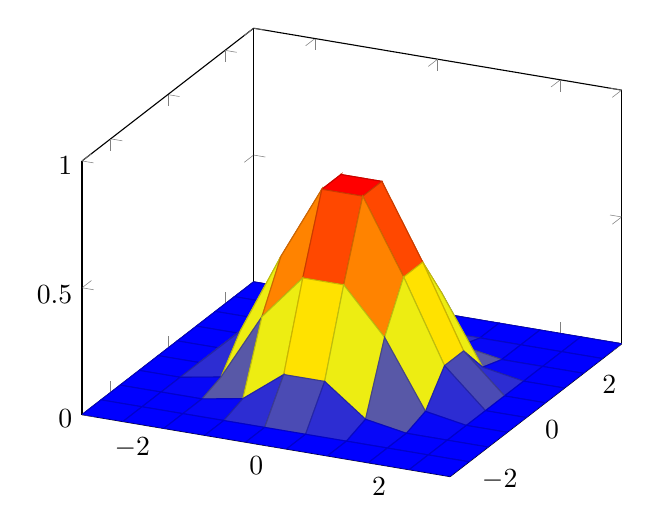
\begin{tikzpicture}[]
    \def\r(#1,#2){sqrt((#1)^2 + (#2)^2) / 2}
    \def\K(#1,#2){2 * \r(#1,#2)^3 - 3 * \r(#1,#2)^2 + 1}
    \begin{axis}[
        % xmin=-2.5,xmax=2,
        % ymin=-2.5,ymax=2,
        zmin= 0  ,zmax=1,
        % axis line style={draw=none},
        % axis equal image,
    ]
    \addplot3[
        surf,
        domain=-3:3,
        samples=10
    ]
    % K(x,y) = 2r^3 - 3r^2 + 1 if r < 1 else 0
    % r = sqrt(x^2 + y^2) / R
    % R = desired radius, lets use 2
    % therefore we get:
    % r = sqrt(x^2 + y^2) / 2
    % K(x,y) = sqrt(x^2 + y^2) / 2 < 1 ? 2 * (sqrt(x^2 + y^2) / 2) ^ 3 - 3 * (sqrt(x^2 + y^2) / 2) ^ 2 + 1 : 0
    {\r(x,y) < 1 ? \K(x,y) : 0};% < 1 ? 2 * r(x,y) ^ 3 - 3 * r(x,y) ^ 2 + 1 : 0};
    \end{axis}
\end{tikzpicture}
\pgfmathdeclarefunction{gauss}{1}{%
    \pgfmathparse{1/(#1*sqrt(2*pi))*exp(-(x^2)/(2*#1^2))}%
}
\pgfmathdeclarefunction{gauss2}{1}{%
    \pgfmathparse{1/(#1*sqrt(2*pi))*exp(-((x)^2 + (y)^2)/(2*#1^2))}%
}
\begin{tikzpicture}[]
    \begin{axis}[
        % xmin=-2.5,xmax=2,
        % ymin=-2.5,ymax=2,
        zmin= 0  ,zmax=1,
        % axis line style={draw=none},
        % axis equal image,
    ]
    \def\r(#1,#2){sqrt((#1)^2 + (#2)^2) / 2}
    \addplot3[
        surf,
        domain=-3:3,
        samples=40
    ]
    {\r(x,y) < 1 ? 1.6666 * gauss2(2/3) : 0};
    \end{axis}
\end{tikzpicture}
\begin{tikzpicture}
    \begin{axis}[every axis plot post/.append style={
        ultra thick, samples=100, domain=-2.5:2.5, mark=none}]
        \addplot {abs(x) < 2 ? 1.6666 * gauss(2/3) : 0};
        \def\r(#1){abs(#1) / 2}%
        \addplot[color=red, dotted]{
            \r(x) < 1 ? 2*(\r(x))^3-3*(\r(x))^2+1 : 0
        };
    \end{axis}
\end{tikzpicture}
\end{minipage}


\subsubsection*{Combined}
\begin{minipage}{.55\textwidth}
    Combining shattering and coaxing, we obtain a somewhat reliable way of generating streamlines according to the footprint left behind by the last frame.
    The seeds created during the shatter process all lie inside the "valley" left behind by the previous streamline path.
    Due to the coaxing function of the modified energy measure,
    it is unlikely that they will leave this valley without a change in the field forcing them to.
\end{minipage}
\begin{minipage}{.45\textwidth}
    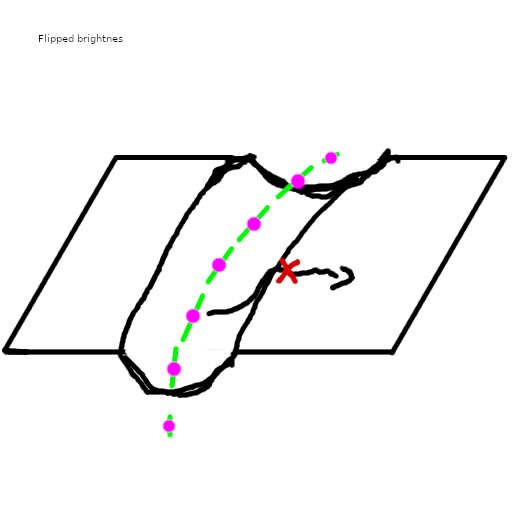
\includegraphics{figures/SL_bump2.png}
    \captionof{figure}{The Fragments' seeds (magenta) "trapped" inside the footprint of previous line}
\end{minipage}
Due to the seeds being held in place in this way, it is very likely for them to re-join to form the same lane they originated from.
If the field changes drastically in this region, the seeds can not fully connect to each other anymore, and will instead gravitate to a different footprint,
forming long patches of coherent lines with interconnections between different paths.
